\section{Unified Process} \label{sec:UP}
En objektorienteret softwareudviklingsproces er Unified Process (UP), som definerer hvem, hvad, hvornår og hvordan softwaren udvikles. UP er bygget om omkring iterationer, hvor softwareudviklingsprocessen deles op i mindre projekter. Dette gøres da det forventes, at fejl opdages hurtigere og er lettere at løse, hvilket ofte medfører, at projekter gennemføres med succes. Hvert projekt er en iteration og opdeles i arbejdsmængder, såsom krav, analyse, design, implementering og test. Denne arbejdsmængde opdeles yderligere i fire faser, herunder opstart, udarbejdelse, konstruktion og overgang, hvor hver fase afsluttes med en milepæl. Hver fase har en eller flere iterationer. Antallet af iterationer afhænger af projektets størrelse. De forskellige faser overlappes i forbindelse med projektets fremskreden og arbejdsmængden ændres.\cite{Arlow2002} Opdeling af projektet og arbejdsmængden ud fra UP fremgår af \autoref{fig:UP}

\begin{figure} [H]
\centering
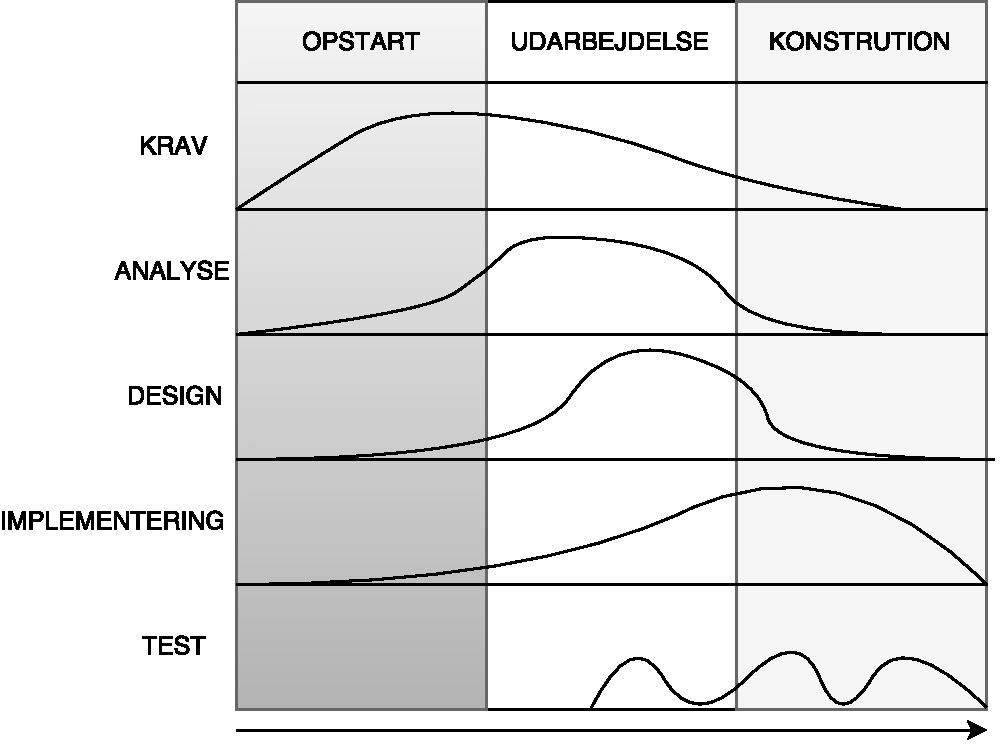
\includegraphics[width=0.8\textwidth]{figures/UP}
\caption{UP struktur. X-aksen viser tiden over projektet opdelt i opstart, udarbejdelse og konstruktion. Y-aksen viser projektets faser, herunder krav, analyse, design, implementering og test. Kurverne viser arbejdsmængden. Revideret \cite{Arlow2002}}
\label{fig:UP}
\end{figure} 

\noindent
Af \autoref{fig:UP} fremgår softwareprocesudviklingen i dette projekt. Opstart og udarbejdelse anvendes med henblik på den senere implementering i konstruktionsfasen. Den sidste fase, overgang, er udeladt af dette projekt, da der kun udvikles en prototype. \fxnote{Skal ændres lidt til hvis vi oplever fejl}

%\section{Software Development Lifecycle}
%Software development lifecycle (SDLC) er en række trin, der kan følges, til udvikling af softwaresystemer for at skabe struktur over arbejdsprocessen. Der er forskellige typer af modeller indenfor SDLC, og dermed forskellige fremgangsmåder for, hvordan processen i softwareudviklingen kan foregå. Eksempler på SDLC-modeller, som anvendes i virksomheder, er vandfaldsmodellen, spiralmodellen og V-modellen. En typisk SDLC-model indeholder stadierne; planlægning, definering, design, implementering, test og brug af systemet.\cite{Jain2011}
%
%\subsection{Vandfaldsmodel} \label{sec:vandfald}
%Vandfaldsmodellen er den ældste og mest brugte SDLC model til udvikling af softwaresystemer. Modellen følger fem faser; analyse og kravspecifikationer, design, implementering, test samt vedligeholdelse. Disse faser gennemgås og dokumenteres enkeltvis førend næste fase påbegyndes. Dette bidrager til at sikre kvaliteten af systemudviklingen. Ved vandfaldsmodellen kan der dog også opstå problematikker i forhold til fejl. Disse fejl kan eksempelvis opstå i første fase, men først opdages i fjerde fase, hvorfor faserne derved skal gennemgås igen.\cite{Alshamrani2015,Bassil2012} Af \autoref{fig:vandfaldsmodel} fremgår vandfaldsmodellen med de fem faser. 
%
%\begin{figure} [H]
%\centering
%\includegraphics[width=0.8\textwidth]{figures/vandfaldsmodel}
%\caption{Vandfaldsmodellens fem faser bestående af analyse og kravspecifikation, design, implementering, test samt vedligeholdelse. Revideret \cite{Alshamrani2015,Bassil2012}.}
%\label{fig:vandfaldsmodel}
%\end{figure} 
%
%\noindent
%Den første fase, analyse og kravspecifikationer, er en omfattende analyse samt beskrivelse af systemets formål. Herunder opstilles funktionelle og non-funktionelle krav, der beskriver, hvilke funktioner samt begrænsninger systemet burde have. Under første fase udarbejdes ligeledes use-case diagrammer i sammenhæng med de funktionelle krav. Efter analyse og kravspecifikationer forekommer designet af systemet. I denne fase planlægges og designes en softwareløsning baseret ud fra første fases kravspecifikationer. Herunder udvælges blandt andet algoritme design, software arkitektur design, databasedesign samt definition af datastruktur. Tredje fase indebærer implementeringen. Denne fase har til formål at implementere og konvertere de opstillede kravspecifikationer samt design fra tidligere faser til et system. Denne konvertering foregår gennem programmering. Den fjerde fase omhandler test og kontrol af softwareløsningen i forhold til de opstillede kravspecifikationer. Vedligeholdelsesfasen, der er den sidste fase, indebærer eventuelle ændringer og forbedringer af softwaresystemet efter det er frigivet.\cite{Alshamrani2015,Bassil2012}








